\scanpage{363}
\uline{(Th) Dold Puppe}\quad Ann Inst Fourier.
\mspage{2}
\[
L_r\operatorname{Sym}^{*}_{\mathbb Z}\simeq L_r\mathbb Z[\qquad]
\]
$\Gamma$

$M_\bullet$ un \inserted{\uline{complexe de} chaines de} $A$-modules
\margin{du moins pour $M$ concentré en un seul degré}

\deleted{$K(M_\bullet)$}

Def
\[
\begin{gathered}
L_{\unsure{i|*}}\mathbb ZM_*=H_i(M_*)\\
\rotatebox{90}{$\approx$}\\
L_i(\operatorname{Sym}\unsure{)|/}M_*)
\end{gathered}
\]
\margin{D'où une graduation (dite la graduation par le poids sur l'homologie des esp d'E.M).}

\uline{Pt clef}: Th de Dold Thom:

$X$ un espace
\margin{$\mathrm{SYM}^{\infty}X$\par
$\cdot\cup X\cup X^{(2)}\cup X^{(3)}\ldots$}
\diagram{\begin{tikzcd}[column sep=small,execute at end picture={\draw (dt.center) ellipse (1.5 and .4);}]
X_{\bullet}\arrow[r]&|[alias=dt]|\pi_i\mathrm{SYM}^{\infty}X&\simeq H_iX
\end{tikzcd}}
Satisfait aux \deleted{\unsure{ax}} \inserted{axioms} Eilenberg-Steenrod
\margin{$\mathbb ZX$\par$\pi_i\underline{ZX}$}
\figure{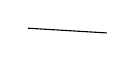
\begin{tikzpicture}\draw (0,0)--(1,-.06);\end{tikzpicture}}

\margin{$G=\mathbb Z^{\ell}\times\mathbb Z$}

$X$ un espace de Moore
\diagram{\begin{tikzcd}[execute at end picture={\draw (moore.center) ellipse (1.5 and .4);}]
|[alias=moore]|\mathbb ZM(G,n).
\end{tikzcd}}
\margin{$G$}
\diagram{\begin{tikzcd}[column sep=small,execute at end picture={\draw (symmoore.center) ellipse (1.9 and .4);}]
K(G,n)&\sim&|[alias=symmoore]|\operatorname{Sym}^{\infty}M(G,n)
\end{tikzcd}}
\diagram{\begin{tikzcd}[column sep=small]
H_i(G,n)=\pi_i\mathbb ZK(G,n)&\overset{\text{Dold Thom}}{=}&\pi_i\mathbb Z\operatorname{Sym}^{\infty}M(G,n)\\
&&\pi_i\operatorname{Sym}(\underbrace{\mathbb ZM(G,n)}_{\substack{\unsure{\Downarrow|\simeq}\\K(G,n)}})\arrow[u,"\sim"]\\
&&=L_i\operatorname{Sym}(G)
\end{tikzcd}}
\diagram{\begin{tikzcd}
G\arrow[r]&M(G)
\end{tikzcd}}
\deleted{\diagram{\begin{tikzcd}
\unsure{M(G),M(H)|M(G),M(G)}\arrow[r]&\unsure{\operatorname{Hom}(G,1)}\arrow[d,bend left=15,no head]\\
&\operatorname{Ext}(G,H)
\end{tikzcd}}}
Theoreme de Dold.
\diagram{\begin{tikzcd}
\mathbb Z\operatorname{Sym}^{\infty}X&\operatorname{Sym}\underline{ZX}\arrow[l,"\sim"']
\end{tikzcd}}
\deleted{Free}

Par def
\[
\mathbb ZM(G,n)\sim K(G,n)
\]
\[
H_{n+r}K(M,n)\overset{s}{\simeq}H_{n+r+1}K(M,n+1)
\]
\deleted{$n\leq r\leq2n$}

$r<n$.
\mspage{364}
